\documentclass[10pt,a4paper]{article}

\usepackage[margin=0.72in]{geometry}
\usepackage[T1]{fontenc}
\usepackage[utf8]{inputenc}
\usepackage{lmodern}
\usepackage{microtype}
\AtBeginDocument{\fontsize{9.5pt}{11.4pt}\selectfont}
\usepackage{booktabs}
\usepackage{array}
\usepackage{enumitem}
\usepackage{tikz}
\usetikzlibrary{positioning,arrows.meta,fit,backgrounds,calc}
\usepackage{xcolor}
\usepackage[colorlinks=true,linkcolor=black,citecolor=blue!60!black,urlcolor=blue!60!black]{hyperref}
\usepackage{titlesec}
\usepackage{caption}
\usepackage{multicol}

\titleformat{\section}{\large\bfseries}{\thesection}{0.6em}{}
\titleformat{\subsection}{\normalsize\bfseries}{\thesubsection}{0.6em}{}
\titlespacing*{\section}{0pt}{0.9em}{0.3em}
\titlespacing*{\subsection}{0pt}{0.8em}{0.3em}
\setlist{nosep,leftmargin=1.4em}
\captionsetup{font=small,labelfont=bf}
\setlength{\parskip}{0.22em}
\setlength{\parindent}{0pt}

\newcommand{\todo}[1]{\textcolor{red!70!black}{[#1]}}

\title{\vspace{-1.6em}\large\bfseries
Did the Right Edit Happen in the Right Place?\\
A Research Note on Evaluating Object-Addition Edits in\\ Text-Guided Image-to-Video Generation}
\author{\normalsize Moazzam Umer Gondal \\
\small Prepared for Prof.\ Harry Yang (HKUST) \\
\small November 2026}
\date{}

\begin{document}
\maketitle
\vspace{-2.2em}

\begin{quote}\small
\textbf{Summary.} AlignVid~\cite{alignvid} shows that a training-free attention modulation makes text-guided image-to-video (TI2V) models follow edit instructions more often, measured by yes/no VQA accuracy on the OmitI2V benchmark. The same intervention also increases motion. This note proposes a small, matched study on the \emph{object addition} subset of OmitI2V that scores three things separately: whether the requested object appears inside an annotated intended region, whether the reference image is preserved outside that region, and how much the video moves. It uses DyMoS~\cite{dymos}, a motion method that leaves text attention untouched, and a no-edit control prompt as reference points, and ends with a blinded failure review. The goal is to learn whether the reported VQA gain reflects correct, well-placed edits, and to produce the first region annotations for OmitI2V. No large experiment is required; a pilot fits in a modest GPU budget.
\end{quote}

\section{Background and problem}

In TI2V generation the model receives a reference image and a text prompt and produces a short video whose first frame is the image. AlignVid~\cite{alignvid} identifies \emph{visual dominance}: the reference image spreads the model's attention too thinly (high entropy), which drowns out the text, so edit instructions (``a sunflower grows in front of the house'') are ignored while the video simply animates the input. Its fix, Attention Scaling Modulation, multiplies query or key vectors by $\gamma = 1.35$ in foreground-sensitive transformer blocks during early denoising. On OmitI2V, addition accuracy rises from 68.6 to 73.1 (FramePack) and 71.8 to 79.5 (Wan2.1), with VBench Dynamic Degree rising from 20.1 to 28.5 on FramePack~\cite{alignvid}.

The OmitI2V protocol asks Qwen2.5-VL-32B yes/no questions about the generated video (``Did a sunflower appear in front of the house?''), with the judge seeing only the video and never the prompt, and reports per-sample macro accuracy. Visual quality is Dynamic Degree and Aesthetic Quality; VBench subject and background consistency are deliberately excluded because additions and deletions change the scene by design~\cite{alignvid}. This protocol answers \emph{whether} an edit happened. It does not record \emph{where} the object appeared, \emph{when} it appeared and whether it persisted, or whether the rest of the scene survived. The paper's own judge audit (FramePack~v1 outputs) reports 3.4\% overall error (0.8\% false positives, 2.6\% false negatives) and names two tendencies: a conservative failure mode on small or occluded objects, and a slight positive bias toward endorsing the prompted effect~\cite{alignvid}. Note also that although the judge never sees the prompt, each question names the object and location, so it is told what to look for.

DyMoS~\cite{dymos} tackles a related effect it calls \emph{reference-frame dominance}: generated frames over-attend to the first frame's key tokens, which suppresses motion. It subtracts a constant from those attention logits in the early denoising steps and raises Dynamic Degree on Wan2.1, Wan2.2, CogVideoX and HunyuanVideo-1.5. It reports ViCLIP text--video similarity and a user-study text-alignment score but never evaluates edit-instruction compliance. Under the hood the two methods overlap more than their framing suggests. In Wan2.1, AlignVid scales the image-side query and text-side key of \emph{cross}-attention; in FramePack, which is a single-stream architecture with no cross-attention, it scales the full key tensor of the joint self-attention in the preset blocks, which sharpens the attention over video, reference and text tokens together. DyMoS instead adds a negative offset to the logits of reference-frame keys only, in self-attention, leaving text tokens untouched. On FramePack both methods therefore act on the same video$\to$reference attention map, by different operations; both weaken the image's grip and both increase motion.

This creates a confound that neither paper tests. A video that moves and changes more gives a VLM judge more ``evidence'' that something happened, so a yes/no score could rise partly because of motion rather than because the requested object was correctly added. The opposite confound is already documented: VBench-style consistency metrics reward static video (DEVIL finds a $-0.81$ correlation between subject consistency and dynamics~\cite{devil}), and VLM judges lean toward ``yes'' on object-existence questions~\cite{pope}. As far as I could find, no paper has measured whether VLM-judged edit accuracy on TI2V rises with motion independently of correctness. That is the question this note targets.

\section{Related evaluation protocols}

The pieces needed for a region-aware evaluation exist in neighbouring benchmarks, but none combines them for single-image object addition in TI2V.

\textbf{PIE-Bench}~\cite{piebench} is the image-domain template: 700 images (80 ``add object'') with a hand-drawn mask of the anticipated edit region; PSNR, LPIPS, MSE and SSIM are computed only outside the mask and CLIP similarity inside it. Its lesson: preservation must be reported next to an edit-success metric, since a model that does nothing scores perfectly on preservation.

\textbf{FiVE-Bench}~\cite{five} brings masked metrics to video editing with SAM2 masks and a \emph{paired} VQA check: the judge must answer ``No'' for the source object and ``Yes'' for the target. The paired No/Yes design is a cheap guard against yes-bias. It has only 10 addition videos.

\textbf{PointBench} (Point2Insert~\cite{point2insert}) is the closest structural template: object insertion into video with a specified region, scored by (i)~a geometric point-hit test inside the mask of the newly added object, (ii)~pixel metrics in unedited regions, (iii)~warping error and CLIP temporal consistency, and (iv)~a VLM rubric where the region is drawn as a red box. Its authors report that VLMs \emph{struggle to judge placement} and produce false positives when the object lands just outside the box, which is why placement relies on the geometric check.

\textbf{HOI-Edit}~\cite{hoiedit} is the only work I found that scores I2V outputs region-sensitively: annotated boxes are propagated to generated frames with SAM~2 and the judge sees cropped or boxed frames. It also states the main practical difficulty: I2V models introduce camera drift, so pixel-level background ``freezing'' cannot be guaranteed.

\textbf{CoVEBench}~\cite{covebench} contributes a preservation rubric in which the judge compares two videos and is told to ignore plausible secondary effects the edit logically causes (lighting and shadow shifts, reflections of a new object). I borrow this for the rater guide.

\textbf{VBench}~\cite{vbench} defines Dynamic Degree as a binary static/non-static label per video from the top-5\% RAFT flow magnitudes, so model-level scores carry no information about motion \emph{magnitude}. The VBench authors note that static videos gain an advantage on temporal metrics; DEVIL~\cite{devil} quantifies it. For this study motion must therefore be reported as a continuous quantity, on its own axis.

\textbf{VLM judges.} Object-existence yes-bias is well documented for open VLMs~\cite{pope}, and EditInspector~\cite{editinspector} finds GPT-4o detected only 12\% of the differences between source and edited images. The recurring fixes: box the region in the visual prompt, include a question whose correct answer is ``No'', and add a geometric check independent of the VLM.

\section{Research questions and hypotheses}

\textbf{RQ1.} When AlignVid raises OmitI2V addition accuracy, does the requested object actually appear inside the intended region, and does it persist across frames?
\textbf{RQ2.} How much of the VQA gain survives when motion is held constant, and does a reference-attention intervention with no text-side term (DyMoS) raise the VQA score at all?
\textbf{RQ3.} What does the edit cost in preservation outside the intended region, relative to a no-edit video from the same backbone and seed?

\begin{itemize}
\item \textbf{H1 (edit success is real).} AlignVid raises both VQA accuracy and detector-based in-region appearance rate, and the two agree per sample.
\item \textbf{H2 (motion confound).} Part of the VQA gain is attributable to motion: the DyMoS arm raises VQA accuracy without modifying text cross-attention, or AlignVid's gain shrinks within bins of matched background motion.
\item \textbf{H3 (preservation cost).} Masked LPIPS/DINOv2 distance outside the region is higher under AlignVid than under the unmodified model; comparing against DyMoS at matched motion tells whether this is an edit cost or a motion cost.
\item \textbf{H4 (placement).} For prompts implying a location, AlignVid shifts successes toward in-region additions rather than scattering objects. Onset frame and persistence are recorded as new descriptive quantities.
\item \textbf{H5 (judge false positives rise with motion).} Running OmitI2V's object-presence questions (those whose answer can only be ``yes'' if the new object exists; relation and attribute questions excluded) on no-edit control videos gives a false-positive rate, and that rate rises with the video's motion.
\end{itemize}

\section{Proposed study}

\begin{figure}[t]
\centering
\resizebox{0.88\textwidth}{!}{%
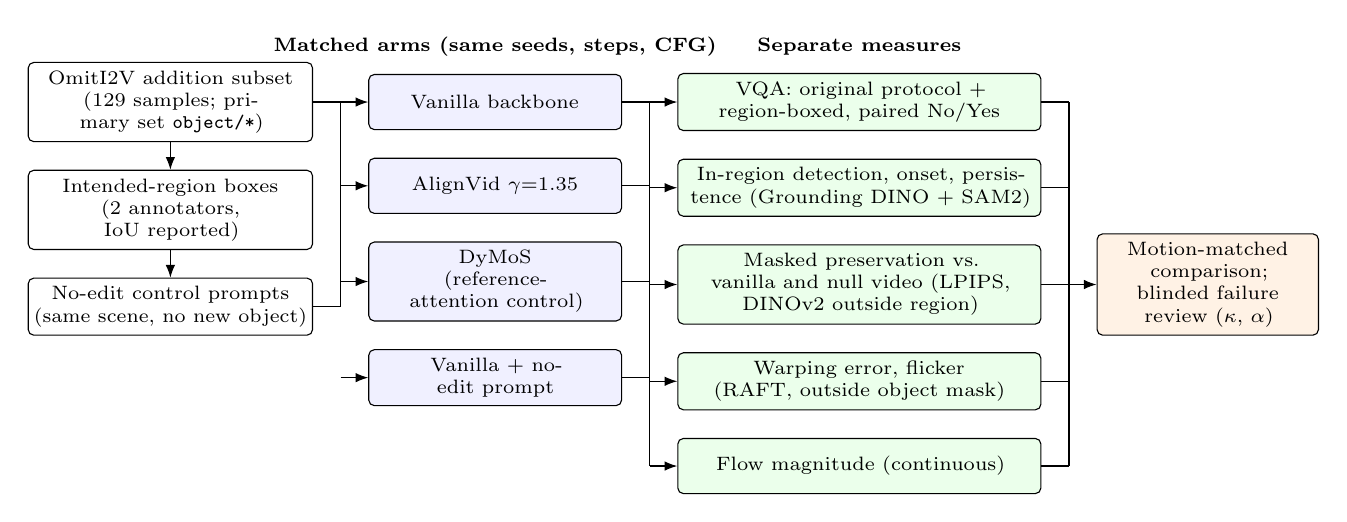
\begin{tikzpicture}[
  node distance=3.5mm and 7mm,
  box/.style={draw,rounded corners=2pt,align=center,font=\scriptsize,inner sep=3pt,minimum height=7mm,fill=white,text width=34mm},
  arm/.style={box,fill=blue!6,text width=30mm},
  meas/.style={box,fill=green!8,text width=44mm},
  lab/.style={font=\scriptsize\bfseries},
  >={Latex[length=1.6mm]}
]
\node[box] (data) {OmitI2V addition subset\\(129 samples; primary set \texttt{object/*})};
\node[box,below=of data] (annot) {Intended-region boxes\\(2 annotators, IoU reported)};
\node[box,below=of annot] (null) {No-edit control prompts\\(same scene, no new object)};

\node[arm,right=of data] (a1) {Vanilla backbone};
\node[arm,below=of a1] (a2) {AlignVid $\gamma{=}1.35$};
\node[arm,below=of a2] (a3) {DyMoS\\(reference-attention control)};
\node[arm,below=of a3] (a4) {Vanilla + no-edit prompt};
\node[lab,above=1mm of a1] {Matched arms (same seeds, steps, CFG)};

\node[meas,right=of a1] (m1) {VQA: original protocol + region-boxed, paired No/Yes};
\node[meas,below=of m1] (m2) {In-region detection, onset, persistence (Grounding DINO + SAM2)};
\node[meas,below=of m2] (m3) {Masked preservation vs.\ vanilla and null video (LPIPS, DINOv2 outside region)};
\node[meas,below=of m3] (m4) {Warping error, flicker (RAFT, outside object mask)};
\node[meas,below=of m4] (m5) {Flow magnitude (continuous)};
\node[lab,above=1mm of m1] {Separate measures};

\node[box,fill=orange!10,text width=26mm,right=of m3] (rev) {Motion-matched comparison;\\blinded failure review ($\kappa$, $\alpha$)};

\coordinate (t1) at ($(data.east)!0.5!(a1.west)$);
\coordinate (t2) at ($(a1.east)!0.5!(m1.west)$);
\coordinate (t3) at ($(m1.east)!0.5!(rev.west)$);

\draw[->] (data) -- (annot);
\draw[->] (annot) -- (null);
\draw (data.east) -- (data.east -| t1);
\draw (null.east) -- (null.east -| t1);
\draw (data.east -| t1) -- (null.east -| t1);
\foreach \a in {a1,a2,a3,a4}{\draw[->] (\a.west -| t1) -- (\a.west);}
\foreach \a in {a1,a2,a3,a4}{\draw (\a.east) -- (\a.east -| t2);}
\draw (a1.east -| t2) -- (a4.east -| t2);
\draw (m1.west -| t2) -- (m5.west -| t2);
\foreach \m in {m1,m2,m3,m4,m5}{\draw[->] (\m.west -| t2) -- (\m.west);}
\foreach \m in {m1,m2,m3,m4,m5}{\draw (\m.east) -- (\m.east -| t3);}
\draw (m1.east -| t3) -- (m5.east -| t3);
\draw[->] (rev.west -| t3) -- (rev.west);
\end{tikzpicture}}
\caption{Study flow. Data and annotations (left) feed four matched generation arms (middle), which are scored by five separate measures (right) and then analysed together.}
\label{fig:flow}
\end{figure}

\subsection{Data and intended edit regions}

I will start from the 129 addition samples in the public OmitI2V release (Apache-2.0), which already provide a prompt, an expected-change string, a \texttt{key} field and 2--6 yes/no questions per sample (the paper's category percentages imply $\sim$122 addition samples; 129 is the count in the released \texttt{meta.json}). The release contains no masks or region annotations, so those are the contribution here. The primary set is \texttt{addition/object/*}, since \texttt{element} additions (logos, text, UI, effects) and \texttt{appearance} additions are not physical-object insertions and would dilute a placement metric; the remaining sub-categories stay as a secondary set so the full 129 remains comparable to the paper. I will verify counts and labels directly in \texttt{meta.json} and flag any anomalies.

\emph{Annotation protocol.} Two annotators independently draw one axis-aligned box per sample on the reference image marking where the prompt implies the object should appear (``a cat on the sofa'' $\to$ the sofa seat), in normalised coordinates since the backbones resize inputs. Each sample gets a location-specificity tag (explicit / implied by scene / unspecified). Samples with no implied location form a ``free placement'' group scored only for presence, preservation and motion. The final box is dilated by 10\% of the shorter image side to form the preservation exclusion zone. Inter-annotator IoU is reported, with IoU $> 0.5$ (the conventional detection threshold, also used by HOI-Edit for its tracking-success criterion~\cite{hoiedit}) as the acceptance bar; disagreements are resolved by discussion. Because both methods increase camera and subject motion, a fixed box would penalise correctly placed objects that move with the scene, so the region is propagated per frame (SAM~2 on an anchor region such as the sofa seat, with a RAFT-based background homography as fallback), and placement is additionally scored over the first frames after onset. Hard cases (small targets, partially hidden placements, objects that must interact with an existing subject) are tagged so the human review includes more of them. Boxes are drawn before any video is generated.

\emph{No-edit control prompts.} For each sample I write a motion-neutral caption of the reference image that mentions no new object. Generated with the same backbone and seed, this video shows the backbone's intrinsic motion and drift when asked for nothing~\cite{hoiedit}. It serves three purposes: a drift reference for preservation, a measure of how much the backbone moves on its own (used in the motion-matched analysis, since it does not depend on the method being tested), and the judge false-positive check for H5.

\subsection{Matched comparisons}

All arms share backbone, resolution, frame count, sampling steps, guidance scale, acceleration settings and 3--5 fixed seeds. Settings follow the released AlignVid code. Where the code differs from the paper text I will report the values actually used: for example, the ``early'' window is implemented as timestep $> 900$, which with the shipped schedules is 10 of 40 steps on Wan2.1-480p but 11 of 25 steps on FramePack at 480p (applied per generation section), against the paper's ``first 30\%''. The FramePack numbers quoted above are for FramePack~v1; its inverted anti-drifting sampling generates the last section first, so for onset and persistence I would use FramePack-F1 (forward sampling) or flag the caveat.

\begin{center}\small
\begin{tabular}{@{}p{3cm}p{6.6cm}p{5.6cm}@{}}
\toprule
Arm & Setting & Purpose \\
\midrule
Vanilla & Backbone defaults from the AlignVid repo & Baseline \\
AlignVid & $\gamma = 1.35$, early-step window, preset foreground blocks & Treatment \\
DyMoS & Published $\gamma/\lambda$ for the backbone, same edit prompt & Reference-attention control (no text-side term) for H2, H3 \\
No-edit control & Vanilla backbone, descriptive no-edit caption & Preservation reference; judge calibration (H5) \\
\bottomrule
\end{tabular}
\end{center}

An optional fifth arm at $\gamma = 1.15$ or $1.25$ (values the paper ablated) would show how the effects scale with $\gamma$. The primary backbone is FramePack, which AlignVid ships ready-made batch scripts for and which is the cheapest of its three backbones. One compatibility issue must be stated. DyMoS's public release currently ships only its Wan2.2-I2V-A14B implementation ($\gamma = 0.6$, first 8 steps); the paper reports settings for Wan2.1-14B ($\gamma = 1.0$, $\lambda = 0.25$), CogVideoX-5B ($\gamma = 0.8$, $\lambda = 0.24$) and HunyuanVideo-1.5, but that code is announced as forthcoming. AlignVid ships FramePack, FramePack-F1 and Wan2.1-I2V-14B. No backbone is shared by both releases, so one method must be re-implemented. DyMoS is a single additive bias on self-attention logits (Eq.~6 of the paper), so my plan is to port it into AlignVid's Wan2.1 fork using the paper's Wan2.1 settings, and run all four arms on Wan2.1-I2V-14B for the review subset. Wan2.1 costs roughly $3.4\times$ FramePack per video, so the full 129-sample vanilla-vs-AlignVid sweep would stay on FramePack, and the Wan2.1 four-arm study would cover the 40-sample review subset. I would not run a cross-backbone control: different frame rates and lengths break both the flow comparison and rater blinding.

\subsection{Separate measures}

The rule I adopt, following PIE-Bench's and PointBench's practice of reporting edit success and preservation as separate numbers~\cite{piebench,point2insert}, is that no single score may absorb the others; Table~\ref{tab:measures} lists each measure with its recipe. Detector thresholds, the value of $k$ and the Grounding DINO text template are fixed before any treatment video is scored.

\begin{table}[!htbp]\centering\small
\begin{tabular}{@{}p{2.6cm}p{7.9cm}p{4.7cm}@{}}
\toprule
Measure & Recipe & Isolates \\
\midrule
Edit success (comparability) & Run the released OmitI2V evaluator unchanged (Qwen2.5-VL-32B, 8\,fps, per-sample macro accuracy) & Direct comparison with the paper \\
Edit success (region-aware) & Same judge; frames with the intended box drawn in red; ``was a new [object] added inside the red box?'' plus a negative question (``is there a [object] anywhere outside the box?'') whose correct answer is No~\cite{point2insert,five} & Yes-bias; out-of-region insertions \\
In-region detection & Grounding DINO~\cite{gdino} on 16 uniformly sampled frames, box threshold raised to 0.4--0.5; present if detected in $\ge k$ of 16 frames ($k = 4$ unless the pilot says otherwise); in-region if at least half the detected box area falls inside the propagated region (centroid-in-box reported as secondary); also onset frame and persistence fraction & Placement, independent of the VLM \\
Object mask & SAM~2~\cite{sam2} seeded with the first confident detection, propagated across frames & Per-frame exclusion mask \\
Preservation & LPIPS~\cite{lpips} (AlexNet) and DINOv2~\cite{dinov2} ViT-B/14 cosine distance outside the union of the dilated region and the object mask, computed (a) between the AlignVid/DyMoS frame $t$ and the vanilla frame $t$ from the same prompt and seed (the direct comparison H3 needs), (b) against the static reference image for the first frames, and (c) against the null-arm frame $t$ as a drift reference; PSNR secondary & Collateral change outside the edit \\
Temporal consistency & RAFT~\cite{raft} flow between consecutive frames with forward--backward occlusion check; warping error and inter-frame flicker outside the object mask; DINOv2 similarity of the object crop across detected frames & Background stability vs.\ new-object stability \\
Motion & Mean and top-5\% RAFT flow magnitude per video, reported as continuous numbers; VBench Dynamic Degree for comparability & Motion as its own axis \\
\bottomrule
\end{tabular}
\caption{Separate measures. Each is reported on its own; none is folded into a composite score.}
\label{tab:measures}
\end{table}

\emph{Motion-matched analysis.} An object appearing is itself optical flow, so grouping videos by their own total flow would partly hide the effect being tested. Videos are therefore grouped by \emph{background} motion: flow computed outside the SAM~2 object mask, and, as a second check, the flow of the no-edit video for the same sample and seed (how much the backbone moves on its own, independent of the method). Vanilla vs.\ AlignVid VQA accuracy is reported within each tercile, paired by sample, with a simple logistic regression of per-question correctness on arm and background flow. The DyMoS arm's VQA accuracy and in-region rate are reported as the no-text-term reference. The H5 false-positive rate on no-edit videos is reported by flow bin. Together these give three independent readings of ``does the gain survive motion matching''.

\subsection{Blinded failure review}

Two raters who did not generate the videos see the reference image, the prompt and one video at a time, with arm identity hidden and order randomised (following VBench~\cite{vbench} and the categorical scheme of EditInspector~\cite{editinspector}); all reviewed arms come from the same backbone at the same resolution and length, otherwise blinding fails. Each video receives a binary success label and exactly one primary failure category: (1)~no change / edit not applied; (2)~wrong object or attribute; (3)~wrong location or scale; (4)~partial or transient appearance (object present only in some frames); (5)~over-editing or unwanted change outside the region; (6)~identity drift of the original scene; (7)~artifacts; (8)~motion-only change (camera or subject motion without the requested object). Categories 4 and 8 are specific to video and, as far as I know, have not been used in published taxonomies. The rater guide includes CoVEBench's instruction to ignore lighting and shadow changes caused by the edit~\cite{covebench}.

A review set of 40 samples $\times$ 3 edit arms $=$ 120 videos is in line with earlier studies and small enough for both raters to label every video. I will report Cohen's $\kappa$ for the binary label (two raters, fully crossed) and Krippendorff's $\alpha$ for the eight-class category, with raw agreement and the count of disagreements, since $\kappa$ intervals are wide at this size~\cite{hallgren}. Thresholds are fixed in advance ($\alpha \ge 0.80$ definite, $0.67$--$0.80$ tentative). Human labels then give per-video precision and recall for both the VLM judge and the detector, extending the paper's own audit (FramePack~v1 only) to a second backbone and to placement.

\section{What would confirm or refute each hypothesis}

\textbf{H1} is confirmed if AlignVid's VQA gain is matched by a similar rise in in-region detection and the two agree per sample (Cohen's $\kappa$ between VLM-yes and detector-in-region $\ge 0.6$); refuted if VQA rises while detection is flat or rises mostly out of region.
\textbf{H2} is refuted, and AlignVid's gain shown to be a real edit effect, if the DyMoS arm stays at baseline VQA and AlignVid's gain holds in every flow bin; confirmed if DyMoS raises VQA with no in-region gain, or the within-bin gain collapses.
\textbf{H3} is confirmed if masked LPIPS/DINOv2 distance is higher for AlignVid than vanilla at matched motion; reinterpreted as a motion cost rather than an edit cost if DyMoS shows the same degradation at the same flow level.
\textbf{H4} is answered descriptively by the in-region rate per arm plus onset and persistence distributions.
\textbf{H5} is confirmed if the judge's yes-rate on no-edit videos rises across background-motion terciles; refuted if it is flat. The paper's 0.78\% addition false-positive rate is quoted only as context, since it is computed over all audited questions rather than over negatives, and the audit's sample size is not stated.
Any outcome adds to, rather than contradicts, the published claims: the paper measured edit compliance and motion; this study measures where, how persistently, and at what preservation cost.

\section{Limitations}

\begin{itemize}
\item \textbf{Preservation under camera motion.} Two videos with different prompts and the same seed do not produce frame-identical motion, so frame-paired masked LPIPS carries noise. Mitigations: DINOv2 (semantic) alongside LPIPS (perceptual), a first-frames comparison against the static image, and the human ``over-editing'' label as the final say.
\item \textbf{Detector reliability.} Grounding DINO degrades under blur and can hallucinate boxes for absent categories; generated frames are often soft. The $\ge k$-of-16 rule, a hand-labelled validation subset, and measuring the detector's own false-positive rate on no-edit videos are required.
\item \textbf{Sample size.} 129 samples (fewer in \texttt{object}) and 120 reviewed videos give wide intervals on a 4--8 point difference. Results will be effect sizes with intervals; the study establishes a protocol, not a verdict.
\item \textbf{Re-implemented control.} DyMoS on Wan2.1 would be my port of a one-line bias, not the authors' code; I would validate it by reproducing the paper's Dynamic Degree gain on a handful of VBench-I2V prompts before using it. If H100-class compute is unavailable, the four-arm study shrinks further or the DyMoS arm is dropped and H2 rests on the motion-matched analysis alone.
\item \textbf{Annotation subjectivity.} Intended regions are my own labels; IoU is reported and unspecified-location prompts are analysed separately rather than forced into a box.
\end{itemize}

\section{Compute and resources}

\textbf{Available.} I have no dedicated GPU. My own machine is an AMD Ryzen~5 5500U laptop with 16\,GB RAM, enough for the lighter measurement models; for anything heavier I use Google Colab, or Colab Pro when available, which gives intermittent access to an A100-40GB.

\textbf{Needed, and a possible split.} FramePack runs from $\sim$6\,GB VRAM at $\sim$130\,s per video on an H100~\cite{alignvid}, so the 5-sample pilot and the full 129-sample vanilla-vs-AlignVid sweep (one seed, $\sim$260 videos) should fit Colab Pro across a few A100 sessions. The measurement stack (Grounding DINO, SAM~2, LPIPS, DINOv2, RAFT) fits a 16\,GB card and could run on Colab. The judge would be the first bottleneck: Qwen2.5-VL-32B needs $\sim$80\,GB in bf16, so one option is an API-served Qwen model, cross-checked against the 32B judge on a subset. The Wan2.1 four-arm study (40 samples $\times$ 4 arms $\times$ 3 seeds $=$ 480 videos at $\sim$446\,s each, roughly 60 H100-hours on a 40--80\,GB GPU) is beyond Colab, and would need lab compute; I have scoped the FramePack part so that useful results exist on their own, and the split can be adjusted to whatever resources make sense.

\textbf{Pilot.} First step regardless: a 5-sample pilot on Colab (vanilla vs.\ AlignVid, one seed) to confirm the released scripts run and the region-boxed VQA and detector behave sensibly.

\scriptsize
\begin{multicols}{2}
\begin{thebibliography}{99}
\setlength{\itemsep}{0pt}

\bibitem{alignvid} Y.~Liu, W.~Shu, Z.~Huang, H.~Zheng, Y.~Wang, M.~Zhang, J.~Zhu, S.-N.~Lim, H.~Yang. AlignVid: Taming Visual Dominance via Training-Free Attention Modulation in Text-guided Image-to-Video Generation. \emph{ICML}, 2026. arXiv:2512.01334. Code and OmitI2V: \url{https://github.com/LAW1223/AlignVid}.

\bibitem{dymos} W.~Jeon, S.~Park, S.~Shin, S.~Lee, H.~Jeong, H.-G.~Jeon. Rebalancing Reference Frame Dominance to Improve Motion in Image-to-Video Models (DyMoS). \emph{NeurIPS}, 2026. arXiv:2605.19398. Code: \url{https://github.com/shoxedqBbB/DyMoS}.

\bibitem{piebench} X.~Ju, A.~Zeng, Y.~Bian, S.~Liu, Q.~Xu. Direct Inversion: Boosting Diffusion-based Editing with 3 Lines of Code (PIE-Bench). \emph{ICLR}, 2024.

\bibitem{five} M.~Li et al. FiVE-Bench: A Fine-grained Video Editing Benchmark for Evaluating Emerging Diffusion and Rectified Flow Models. \emph{ICCV}, 2025. arXiv:2503.13684.

\bibitem{point2insert} Y.~Zhou, X.~Yang, B.~Zi, et al. Point2Insert: Video Object Insertion via Sparse Point Guidance (PointBench). arXiv preprint 2602.04167, 2026.

\bibitem{hoiedit} J.~Gao, Q.~Chen, Y.~Peng, Y.~Liu. Taming I2V Models for Image HOI Editing: A Cognitive Benchmark and Agentic Self-Correcting Framework (HOI-Edit / HOI-Eval). \emph{ICML}, 2026. arXiv:2606.19073.

\bibitem{covebench} J.~Wu, J.~Wang, Y.~He, et al. CoVEBench: Benchmarking Compositional Video Editing with Fine-grained Diagnostics. arXiv:2606.08415, 2026.

\bibitem{vbench} Z.~Huang et al. VBench: Comprehensive Benchmark Suite for Video Generative Models. \emph{CVPR}, 2024.

\bibitem{devil} M.~Liao et al. Evaluation of Text-to-Video Generation Models: A Dynamics Perspective (DEVIL). \emph{NeurIPS}, 2024. arXiv:2407.01094.

\bibitem{pope} Y.~Li et al. Evaluating Object Hallucination in Large Vision-Language Models (POPE). \emph{EMNLP}, 2023. arXiv:2305.10355.

\bibitem{editinspector} R.~Yosef, Y.~Bitton, D.~Lischinski, M.~Yanuka. EditInspector: A Benchmark for Evaluation of Text-Guided Image Edits. \emph{ACL}, 2025. arXiv:2506.09988.

\bibitem{hallgren} K.~A.~Hallgren. Computing Inter-Rater Reliability for Observational Data: An Overview and Tutorial. \emph{Tutorials in Quantitative Methods for Psychology}, 8(1):23--34, 2012.

\bibitem{gdino} S.~Liu et al. Grounding DINO: Marrying DINO with Grounded Pre-Training for Open-Set Object Detection. \emph{ECCV}, 2024. arXiv:2303.05499.

\bibitem{sam2} N.~Ravi et al. SAM 2: Segment Anything in Images and Videos. \emph{ICLR}, 2025. arXiv:2408.00714.

\bibitem{lpips} R.~Zhang, P.~Isola, A.~Efros, E.~Shechtman, O.~Wang. The Unreasonable Effectiveness of Deep Features as a Perceptual Metric (LPIPS). \emph{CVPR}, 2018.

\bibitem{dinov2} M.~Oquab et al. DINOv2: Learning Robust Visual Features without Supervision. \emph{TMLR}, 2024.

\bibitem{raft} Z.~Teed, J.~Deng. RAFT: Recurrent All-Pairs Field Transforms for Optical Flow. \emph{ECCV}, 2020.

\end{thebibliography}
\end{multicols}

\end{document}
